% Muster für die Seminarausarbeitung
% HPI Potsdam

\documentclass[11pt, a4paper]{article}

\usepackage[english]{babel}
\usepackage[utf8]{inputenc} %Korrekte Kodierung der Umlaute nach UTF-8
\usepackage[T1]{fontenc} %Korrekte Kodierung der Umlaute nach UTF-8
\usepackage{makeidx} %Zur automatischen Indexerstellung
\usepackage{amsfonts}
\usepackage{mathtools}
\usepackage{amssymb}
\usepackage{epsfig}   % Zum Einbinden von Bildern
\usepackage{url}      % Korrekter Satz von URLs
\usepackage{color}    % Verwendung von Farben
\usepackage{listings} % Korrekter Satz von Listings und Quellcode
%\usepackage[parfill]{parskip}


%Hilfs-Fonts - ohne Serifen (hier für Tabellen)
\newfont{\bib}{cmss8 scaled 1040}
%\newfont{\bibf}{cmssbx8 scaled 1040}

\definecolor{lightgray}{gray}{0.85}
\DeclareMathOperator*{\argmax}{\arg\!\max}
\DeclarePairedDelimiterX\Set[2]{\lbrace}{\rbrace}%
 { #1 \,\delimsize|\, #2 }
 \numberwithin{equation}{section}

\setlength\parindent{24pt}

%Seitenformat-Definitionen
\topmargin0mm
\textwidth147mm
\textheight214mm
\evensidemargin5mm
\oddsidemargin5mm
\footskip19mm
\parindent=0in

\makeindex % legt das Index-File an


\begin{document}

\begin{titlepage}
  \begin{center}
    \mbox{}
    \vspace{1cm}

    {\huge Match Forrest, Match! \\[1em] {\LARGE Creating a unified dataset of Movies}}

    \vspace{4cm}

    Seminar paper for \\[1em]
    {\large \sc Semantic Multimedia 2014 - A LOD of Movies} \\[1em]
    Summer Semester 2014 \\[1em]
    Hasso-Plattner-Institut for Softwaresystemtechnik GmbH \\[1em]
    University Potsdam

    \vspace{3cm}

		Authors:

    \vspace{1em}

		{\Large Tanja Bergmann} \\
		{\Large Stefan Bunk} \\
		{\Large Tim Draeger} \\
		{\Large Dominik Müller} \\
		{\Large Ricarda Schüler}

    \vspace{3em}

    August 19th, 2014
  \end{center}
\end{titlepage}


\setcounter{page}{1}

% Zweite Seite = Kurzzusammenfassung
\begin{abstract}
\noindent

The world wide web contains lots of pages about movies, but most of them only offer unstructured content.
This paper describes the aggregation and linkage of movie data from different online movie data sources to a unified, linked open data set.
Therefor, the IMDb, TMDb, OFDb and Freebase are used.
Because one movie can exist in multiple of these data sources, the system has to recognize those movies and match them to one entity.
Entities have different representations in different data sources, this is why a matching algorithm has to be developed.
The matching algorithm presented in this paper uses the overlap of actors to determine which movies should be matched.
The algorithm is explained and evaluated.
Results show a high precision, while still maintaining a good recall.
Besides, the system updates all movies periodically, so that the resulting data set is always up-to-date.

\bigskip

\end{abstract}

\newpage

% Dritte Seite = Inhaltsverzeichnis
\tableofcontents

\newpage

%!TEX root = ../lod-group1.tex
\section{Introduction}
\label{sec_introduction}

The internet contains vast amounts of information on all sorts of topics, movies being one of those.
Should a user search for details on a certain movie, all they have to do is enter its title in the search field of an online movie database and they are presented with a lot of data.
But what if a user does not know the movie's title and doesn't even remember its director or the actors which starred in it?

If users only know some plot points and try to find the corresponding movie's title, they might have to manually sort through hundreds of movies since most online databases don't provide a proper interface for such queries, even if the data is actually available to them.
This problem can be solved by creating a linked open movie database from the data in those online movie databases which should contain traditional data such as the movie's actors or its release data, but also semantic information such as the location where it is set and the major plot points.
This approach was implemented and is presented in this paper.

Every online database contains some information which is not found in others.
So, building a complete database requires gathering data from multiple sources.
The data sources which were used in this project are described in Chapter \ref{subsec_method_datasources} and the categories of data are shown in Chapter \ref{subsec_method_ontology}.
The system's architecture can be found in Chapter \ref{subsec_method_architecture} and the acquisition of the data is covered in Chapter \ref{subsec_method_triplification}.

If there is movie data from different sources, this data needs to be matched so that the linked database knows that both sets of data actually belong together.
Since some movies may have different titles in different data sources, devloping a matching algorithm is not trivial.
This paper details the matching algorithm in Chapter \ref{subsec_method_matching} and evaluates it in Chapter \ref{subsec_evaluation_matching}.

Users often want information on recently released movies because they might wish to decide if those are worth watching in cinema.
Thus, an updating strategy needs to be developed to keep the databases' contents up-to-date.
The stratgey which was implemented is described in Chapter \ref{subsec_method_updating}.

Possible uses for the application of such a linked open movie database include semantic search, explorative search or recommender systems.

This paper details related work in Chapter \ref{sec_related_work}.
Finally, Chapter \ref{sec_conclusion} concludes the paper with an outlook on potential development in the future.
\newpage
%!TEX root = ../lod-group1.tex
\section{Related Work}
\label{sec_related_work}


Triplification (http://linkedmdb.org/), Referenz zur Triplification http://triplify.org/Challenge/ von Movies

Oktie Hassanzadeh and Mariano Consens. Linked Movie Database
\url{http://ceur-ws.org/Vol-538/ldow2009_paper12.pdf}

Hassanzadeh and Consens tried to unify multiple sources of movie data (among them IMDb and Freebase) into an open linked data set.
They utilize approximate string matching methods on movies' titles to find sameAs relation between movies of different sources.
Hassanzadeh and Consens measured the accuracy of their method when using edit similarity, Jaccard or WeightedJaccard, as well as other measures used in information retrieval for string matching.

Leveraging Usage Data for Linked Data Movie Entity Summarization 
\url{http://arxiv.org/abs/1204.2718}

Thalhammer et al. propose an approach to find features which are important for identifying a certain entity in a linked data set.
They do this to allow a summarization of an entity according to only some of its features which is then used to measure similarity to other entities.
Thalhammer et al. focus on the movie domain for their example similarity measures.

T. Berners-Lee. Linked Data, Design Issues.
\url{http://www.w3.org/DesignIssues/LinkedData.html}, 27 July 2006.

Berners-Lee defines four rules to properly defining linked open data.
He proposes to use URIs as names for things, and to use HTTP URIs to allow people to look these up.
Additionally, Berners-Lee states that useful information using certain standards should be provided and that other links to other URIs should be included.

\newpage
\section{Method}
\label{sec_method}

\emph{Match Forrest, Match!} is a system which creates an unifed dataset of movies from different datasources.
In the following, the approach to created this unifed dataset is explained in detail.

\subsection{Data Sources}
\label{subsec_method_datasources}

\emph{Match Forrest, Match!} is built on four different data sources.

The first data source is the \textit{Internet Movie Database (IMDb)}\footnote{\url{http://www.imdb.com/}}.
This data source contains more than 274,000 movies and more than 365,000 people.
%TODO SOURCE ^
To get the individual movie resources, the system has to crawl HTML pages.
While the content in \textit{IMDb} is mostly user-generated, it has to go through multiple consistency checks, performed by professionals \cite{IMDb_DataCreation}.
Thus, we can assume that the data is more likely to be correct when compared to data from entirely user generated data sources.

Another big movie platform is \textit{Freebase}\footnote{\url{http://www.freebase.com/}}.
\textit{Freebase} is a connected user-generated open database, which contains a lot of links to other platforms.
It contains more than 250,000 movies and more than 430,000 people.
%TODO SOURCE ^
\textit{Freebase} offers a MQL API and a Topic API, which can be queried to get movie resources.

\textit{themoviedb.org (TMDb)}\footnote{\url{http://www.themoviedb.org/}} is a movie database which contains a lot of images.
It also offers an API to send requests for movie resources.
\textit{TMDb} is a collection of more than 171,000 movies and 605,000 people.
%TODO SOURCE ^
\textit{TMDb} also published diffs, which is helpful to keep all movies from this data source up-to-date.

The last data source the system utilizes is the \textit{Online-Filmdatenbank (OFDb)}\footnote{\url{http://www.ofdb.de/}}.
This data source is specialised on German movies, but also contains international ones.
It contains more than 236,000 movies and 54,000 people.
%TODO SOURCE ^
%TODO ??Table for the numbers instead??
\\ \\
To create a unified dataset of movies, a main data source must be chosen.
This main source is used to match movies from different data sources against it.
For \emph{Match Forrest, Match!} \textit{IMDb} was chosen as the main data source, since it contains more movies than any of the other data sources.
Additionally, \textit{IMDb} is maintained by data editors, which manually add, delete and update the data\footnote{\url{https://uk-amazon.icims.com/jobs/274286/data-editor\%2c-database-content/job}}.

All the other data sources are not maintained by paid professionals or are not as big as \textit{IMDb}.
\\ \\
Some movies from \textit{Freebase}, \textit{TMDb} and \textit{OFDb} already contain links to the correpsonding \textit{IMDb} movie.
This is immensely helpful in the matching process (Chapter \ref{subsec_method_matching}).
%!TEX root = ../../lod-group1.tex
\subsection{Movie Ontology}
\label{subsec_method_ontology}

As described in the previous section, different data sources, each having their own data format, were used in the system \emph{Match Forrest, Match!}.
To create a unified dataset and therefore enable simple querying over all data, an ontology for movies was defined.

This ontology covers movie resources as well as resources which belong to a movie, such as awards.
In general, the defined ontology is based on the DBpedia ontology.
If no DBpedia class or property was present, Freebase classes or properties or newly defined ones were used.

In the following, the defined entities used in the system with their corresponding RDF classes are listed in Table \ref{tab_entities}.

\begin{table}[ht]
	\begin{center}
	\begin{tabular}{ll}
		\textbf{Entity} & \textbf{RDF class} \\ \hline
		Movie & dbpedia-owl:Film \\
		Award & dbpedia-owl:Award \\
		MoviePerson & dbpedia-owl:Person \\
		Character & freebase:film/performance \\
		MovieCharacter & lod:MovieCharacter \\
		Aka (also known as) & lod:Aka \\
		ReleaseInfo & lod:ReleaseInfo \\
	\end{tabular}
	\end{center}
	\caption{Entities with their corresponding RDF classes}
	\label{tab_entities}
\end{table}

Relations between these resources and their pattern for the unique identifiers are shown in Figure \ref{fig_ontology}.
The prefix \textit{lod} was newly defined for this project.

\begin{figure}[h!]
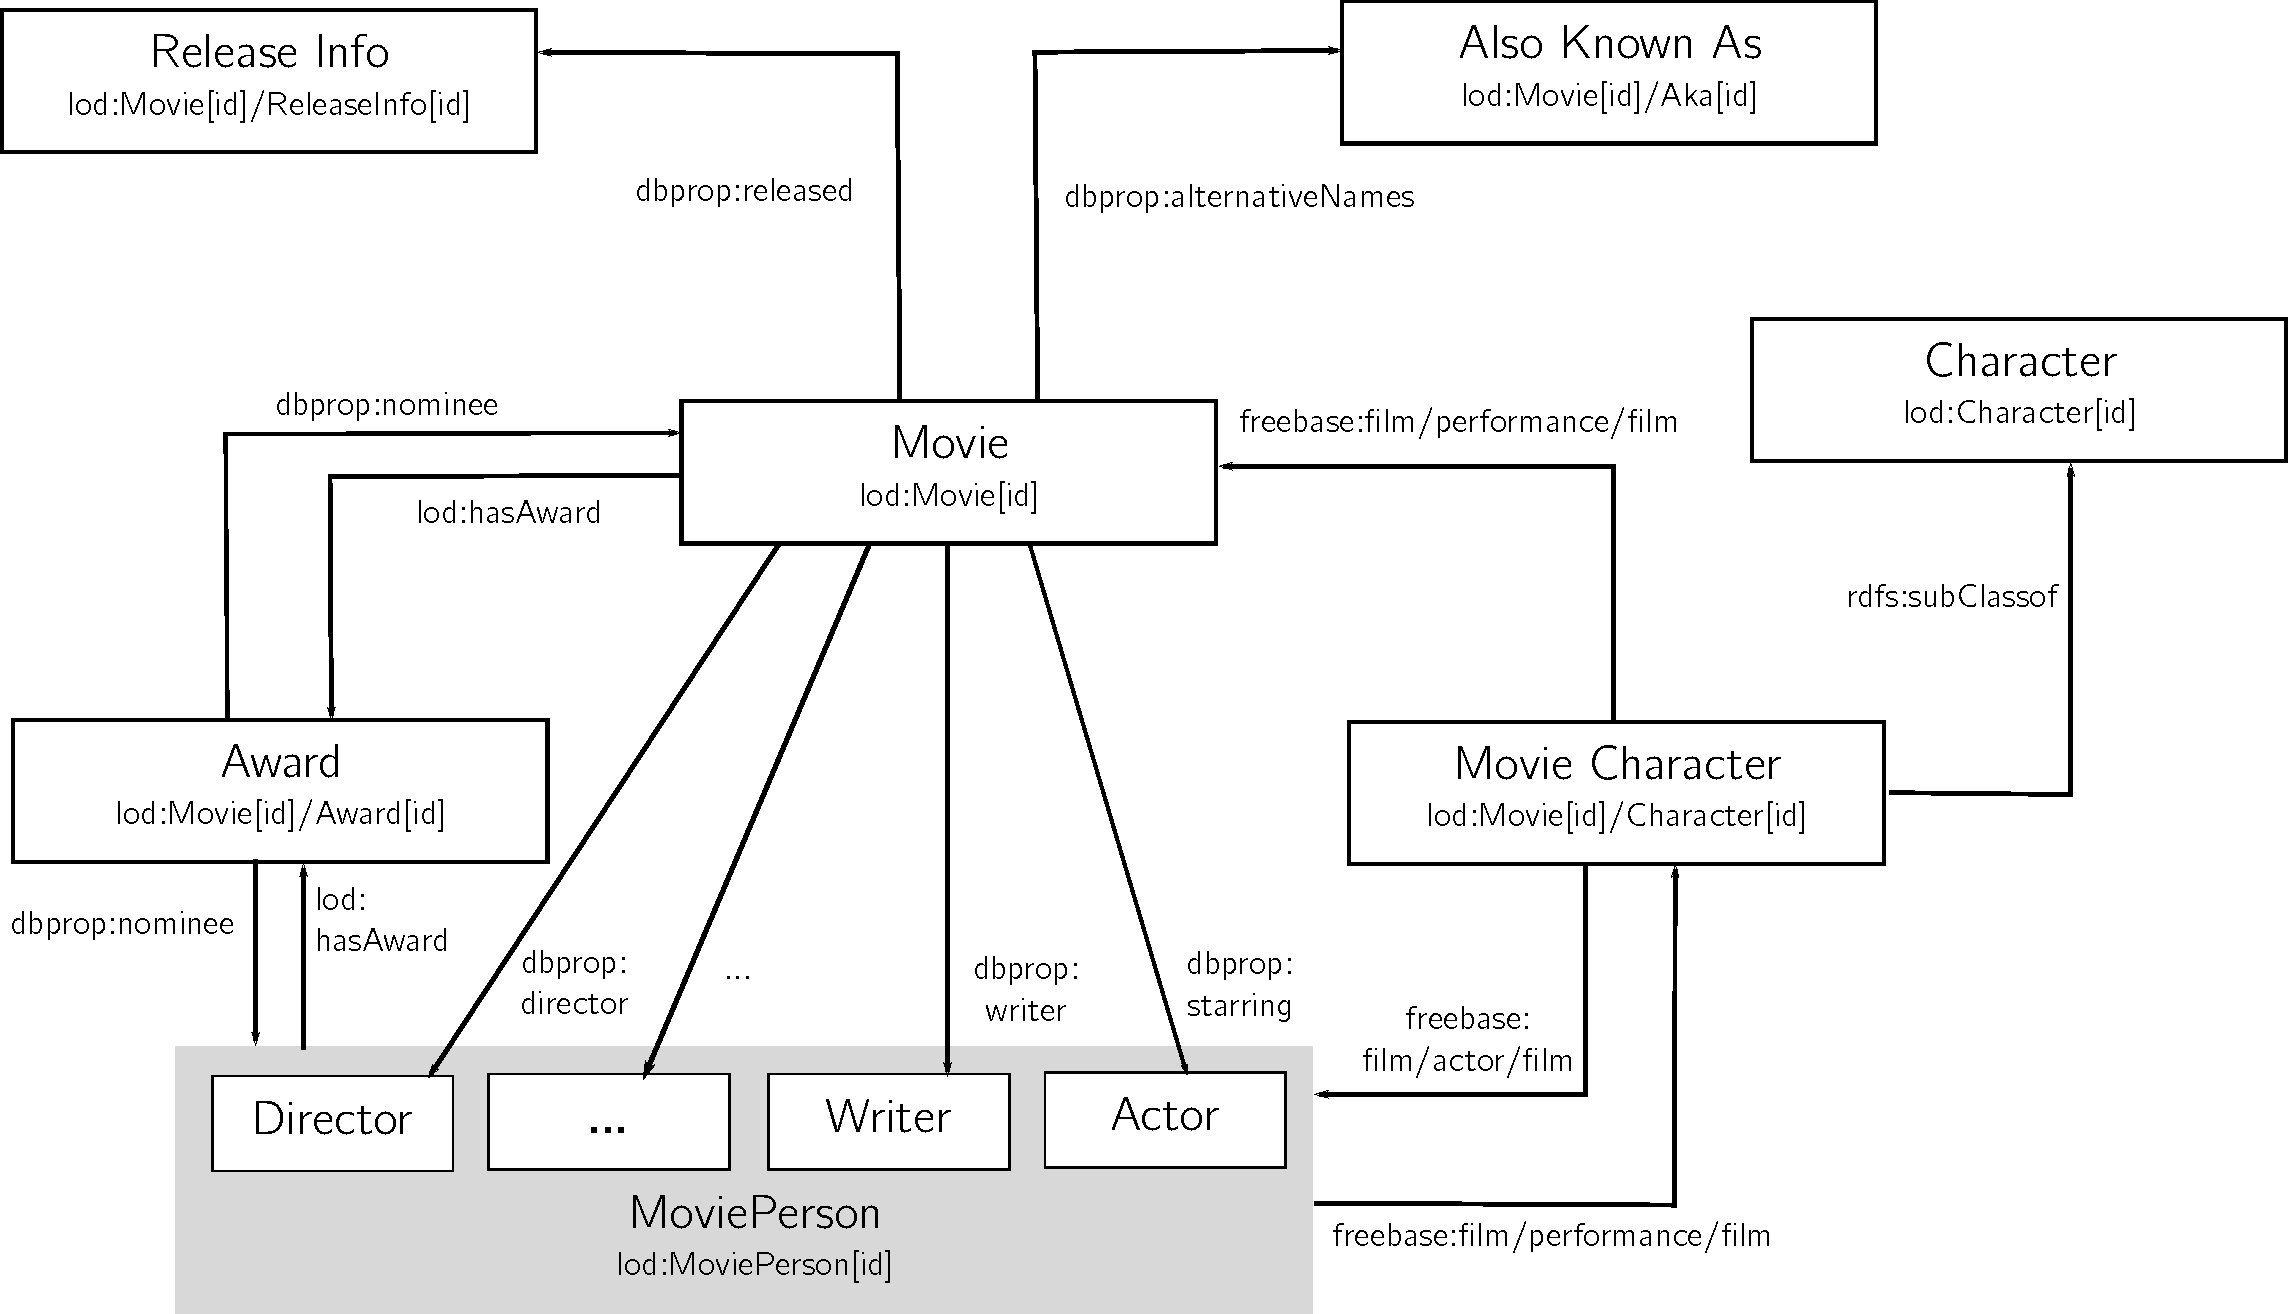
\includegraphics[width=\textwidth]{images/ontology.pdf}
\caption{Movie Ontology. Relations between all resources and their pattern for the unique identifiers.}
\label{fig_ontology}
\end{figure}

A MoviePerson can have multiple sub-types of \textit{dbpedia-owl:Person}, depending on the jobs the person had on any movies they worked on.
As shown in Figure \ref{fig_ontology} a distinction between these jobs (e.g. director, writer, producer) was made.
For example, a person who is a director in one movie and an actor in another movie would have the additional classes \textit{dbpedia-owl:Actor} and \textit{dbpedia-owl:Director}.

A problem, which occured when defining our ontology, was the entity Character.
In the initial definition, there was just one character class, which was connected to the corresponding movie and actor.
The actor also had a connection to the character.
The unique identifier of the character was build from the character's name.

Thus, a character which exists in multiple movies (e.g. "cleaning lady") would be one resource connected to each actor who had ever portrayed this character.
The character also had a list of movies which it occured in.
That way, one could not say which actors played the character in a certain movie.
One such case is an actor who played a certain character in an old movie but also appears in the movie's newer remake.
In the remake, they might play a different character while another actor plays their original character.
An example for this is the movie "Starsky \& Hutch" (2004), which is a remake of the 1970s television series with the same name.
In the movie, both actors which originally portrayed Starsky and Hutch get a cameo appearance alongside the new cast for their old characters.
With the old approach, the system could not know who played the Starsky character in the remake, because all actors who ever played the character are listed.

Therefore, an additional class of MovieCharacter was introduced in the final ontology.
This resource is only connected to one movie and all actors, who played that character in that movie.
The unique identifier of the MovieCharacter is build from the unique identifier of the movie and the character.
The MovieCharacter is a subclass of Character, which describes the general character.
This means, that the unique identifier of the MovieCharacter in the "Starsky \& Hutch" example is "Starksy/Starsky\&Hutch1970" and identifier of Character is "Starksy".
%!TEX root = ../../lod-group1.tex
\subsection{System Architecture}
\label{subsec_method_architecture}

The following section describes the architecture of \emph{Match Forrest, Match!} system.
The central component of the system is the \textit{Task Distributor}.
This component is responsible for managing the other components, \textit{Crawler}, \textit{Triplifier}, \textit{Updater} and \textit{Matcher and Merger}.
It uses a messaging system, which is explained in Section~\ref{subsubsec_messaging_infrastructure}.

\subsubsection{System Overview}
\label{subsubsec_workflow}

The overview about the system can be seen in Figure \ref{fig_architecture}.
The first step to get a movie into the system is always to retrieve the web resource about a movie from one of the data sources.
This step is executed by the Crawler.
This component is responsible for downloading websites or for sending requests to the API a data source might provide.

Once the page is downloaded, the Triplifier can triplify the resource.
This means that it extracts the information from the resource (usually in HTML or JSON format) and creates triples according to a certain ontology.
The ontology is described in Section~\ref{subsec_method_ontology}.

The component Matcher and Merger is in charge of matching and merging two movies from different data sources, so they can only be found once in the resulting dataset.
This is the crucial step in creating a clean dataset
.
This component is explained in detail in Section~\ref{subsec_method_matching}.

The Updater, described in Section~\ref{subsec_method_updating}, ensures that the existing movies are always up-to-date and that new movies are in the system.

The triple store \emph{Virtuoso}\footnote{\url{http://virtuoso.openlinksw.com/}} is used to store the resulting triples.
To distinguish between the sources of the different triples, triples from each data source are stored in a distinct graph named after the source.
Thus, there are four graphs in the triplestore: IMDb, Freebase, TMDb and OFDb.

\begin{figure}[ht]
  \begin{center}
  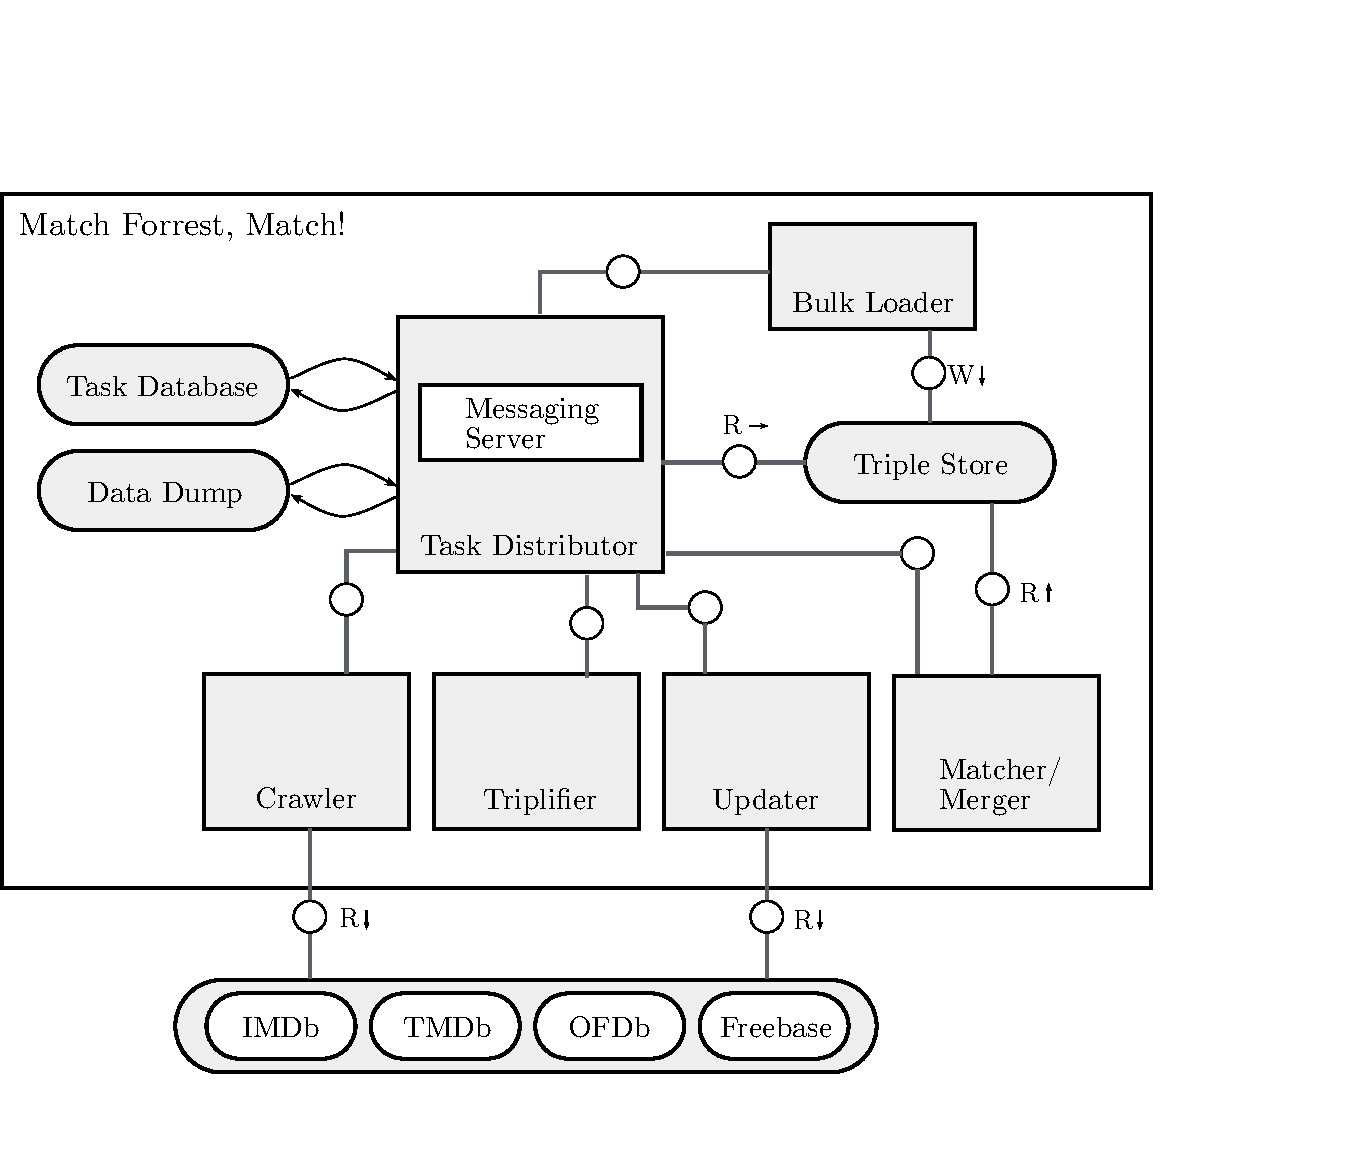
\includegraphics[width=0.7\textwidth]{images/architecture.pdf}
  \end{center}
  \caption{Architecture of \emph{Match Forrest, Match!}. The central component of the system is the Task Distributor, which is responsible for managing the other components, Crawler, Triplifier, Updater and Matcher and Merger.}
  \label{fig_architecture}
\end{figure}

\subsubsection{Messaging Infrastructure}
\label{subsubsec_messaging_infrastructure}

The process of crawling, triplifying and matching a movie resource takes a lot of time.
This is especially true when there are limits to crawl some web pages, which means that waiting times can occur.
Triplifying and matching needs computational resources.
Because these steps can be done in parallel, a messaging infrastructure was implemented to speed up the process and to avoid crawl limits.

Therefore, the Task Distributor uses \emph{RabbitMQ}\footnote{\url{http://www.rabbitmq.com/}} to coordinate and send created task to multiple workers.

A task consists of the following fields
\begin{itemize}
  \item \textbf{Id}:
  The unique id of the task.
  \item \textbf{Task type}:
   The type of the task.
  Basically there is a type for each of the compontents, controlled by the Task Distributor, for example ``Triplify'' or ``MatchAndMerge''.
  ``Triplify'' is a task executed by the Triplifier component.
  The Matcher and Merger component works on ``MatchAndMerge'' tasks.
  There are also tasks, which combine some steps, e.g. one task which crawls, triplifies and matches a movie. This is important for updating, since then all of them are better done at once.
  \item \textbf{Due date}:
  The date until when the task should be finished.
  \item \textbf{File or URL}:
  The file or url which is needed to execute the task, e.g. a URL to crawl or a JSON file to triplify.
  \item \textbf{Finished:}
  Defines if the task is already done.
  \item \textbf{Graph}:
  The graph in which the resulting triples should be stored.
  \item \textbf{Special flags}:
  Additional information needed when executing a task.
  For example, it could tell whether a certain entity should be deleted from the triple store before storing new triples.
\end{itemize}
Not all fields have to be set, the task type defines which fields are needed.
For example the ``Triplify'' task needs a file, but the ``MatchAndMerge'' task does not.

All tasks are stored in an SQL database and new ones are created by the Updater.
To get an initial dataset, tasks have to be created manually.

The messaging server takes a task from the SQL database and puts it into the messaging queue.
The functionality of the messaging system, is shown in Figure \ref{fig_messaging_infrastructure}.
The new task is then pushed to a worker which is registered on the task queue.
If multiple workers are registered, a free worker is selected by using the round robin principle to perform the next task.
When the worker has finished the task, it sends its answer to the answer queue and waits for the server to acknowledge its work.
The server receives the worker's answer from the answer queue and then stores given triples into the triple store or files into the file system.
When the answer was successfully stored, the server sends his acknowledgement to the worker who forwards the acknowledgement to the task queue.
The task is now successfully executed and the worker can work on the next task in the task queue.
If an acknowledgement takes longer than a certain time, the task would be assigned to another worker.
This ensures that no tasks get lost.
By only sending the acknowledgement after storing the data, it is also ensured that only really finished tasks are considered as finished.

\begin{figure}[ht]
  \begin{center}
  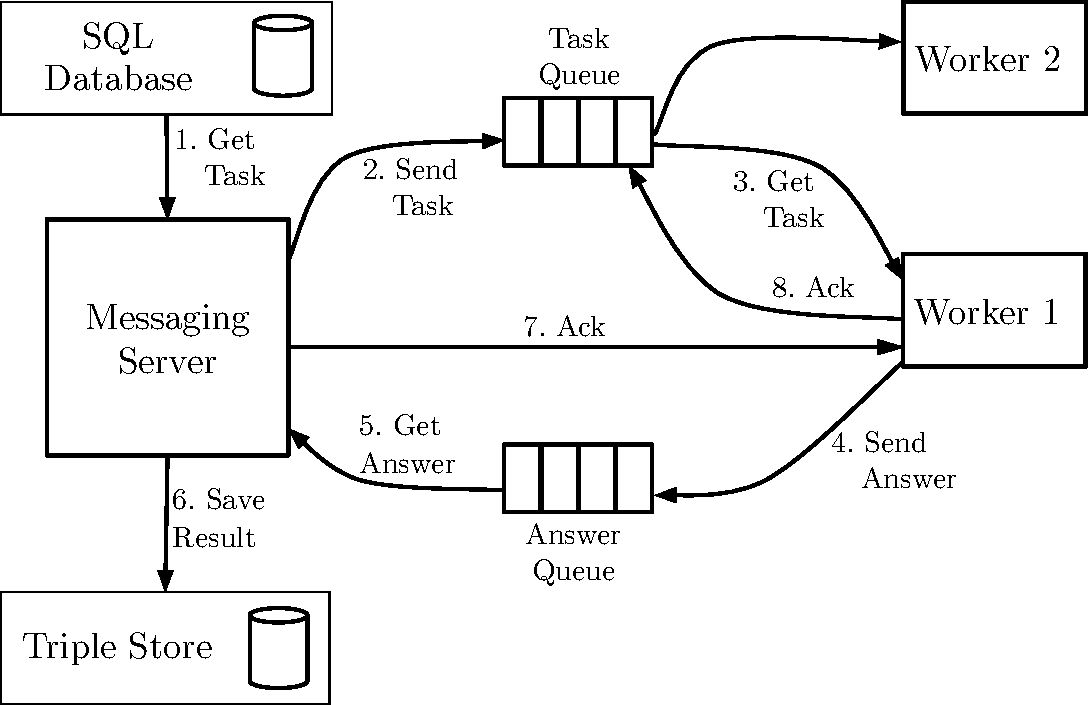
\includegraphics[width=0.7\textwidth]{images/rabbit_mq.pdf}
  \end{center}
  \caption{Messaging Infrastructure using RabbitMQ.}
  \label{fig_messaging_infrastructure}
\end{figure}
%!TEX root = ../../lod-group1.tex
\subsection{Triplification of Movie Resources}
\label{subsec_method_triplification}

Triplification is the step of converting information from a movie resource into triples.
The ontology, defined in Section~\ref{subsec_method_ontology}, is used to generate the triples.

To create triples from the information of a movie resource, the information has to be matched to a corresponding predicate.
For example, the title of the movie "Forrest Gump", displayed on a website, has to be converted into the triple
\begin{center}\emph{<http://movie/Forrest\_Gump> dbpprop:title "Forrest Gump"}.\end{center}
To guarantee this, every data source was analyzed and parsed manually.
So, it is strictly defined which part of a movie resource contains valuable information and which RDF predicate corresponds to the type of information.
%!TEX root = ../../lod-group1.tex
\subsection{Matching}
\label{subsec_method_matching}

The following sections show the approach for matching (i.e. finding the same entity in different datasets) and merging (i.e. integrating two different datasets about the same entity into one.)

\subsubsection{Problem statement}
After loading the initial dataset into the database, the task is to integrate other datasets to create a whole dataset with more information than a single one can provide on their own.
% TODO: Why IMDB?
However, simply dumping the second dataset into the database would lead to duplicated entries and thereby decreasing the overall quality of the database.
Thus, the datasets need to be aggregated and unified by looking for a match for each new entry in the old dataset.
Potentially, this has to be done for matching every entry, such as movies, actors, characters and more but the next parts focus on matching just movies to each other.

A first approach is to match movies only by their name.
However, only using the name as a matching criteria yields multiple problems, such as:
\begin{itemize}
	\item different movies having the same name e.g.
	\begin{itemize}
        \item The Avengers (2012) vs. The Avengers (1998)
        \item Casino Royale (1967) vs. Casino Royale (2006)
    \end{itemize}
	\item same movies having different names in different datasets e.g.
	\begin{itemize}
        \item Spelling errors: Batman vs Badman
        \item Localization: The Internship vs. Prakti.com
        \item Formatting: The Italian Job vs. Italian Job, The
     \end{itemize}
\end{itemize}
Hence, a more sophisticated approach needs to be developed to increase the quality of the dataset.

\subsubsection{Matching using actor overlap}
In general, the matching algorithm must satisfy two requirements:
\begin{enumerate}
	\item{High precision:} A movie should not be matched to a wrong movie, as this decreases the quality of the dataset. We want to find many matches, but it is important not to add too many wrong matches.
	\item{Performance:} With thousand of movies in each new dataset, matching one movie should not take too long.  For Example TMDb has about 170,000 (TODO Check this number) movies to match.
	If each movie takes just 1 minute to match, the whole process for TMDb already takes $171,000~movies * 1 \frac{minute}{movie} * \frac{1}{1440} \frac{days}{minute} \approx 119~days$.
	This is just one data source, and only the current set of movies (remember, there are new movies every day from all data sources, which need to be merged).
\end{enumerate}

This leads to two consequences: First, a certain level of confidence needs to be reached to match two movies to each other. Otherwise, it is impossible to detect movies, which are not matchable, because they are not in the database.
Second, comparing each movie with all movies in the database is not feasible.

This paper proposes the idea to first find a small list of movies that could be a match (henceforth called candidates) and then calculate a score for each of these candidates, which is based on the actors . Details are described in the following paragraphs.

Figure \ref{fig_matching_general} shows the general matching procedure:
First, the algorithm pass through each new movie, that needs to be matched.
For each movie $n_i \in N$ ($N$ is the set of movies, which still needs to be matched), a small set of movies $C_{i}$, that could be a match, is selected.
the next step is to calculate a score, which captures the similarity between $n_i$ and each $m_j \in C_i$.
This score is mostly based on the actor information, which are available about the two movies.
Finally, the movie with the highest score will be chosen, if the score is above a certain threshold.

\begin{figure}[ht]
  \begin{center}
  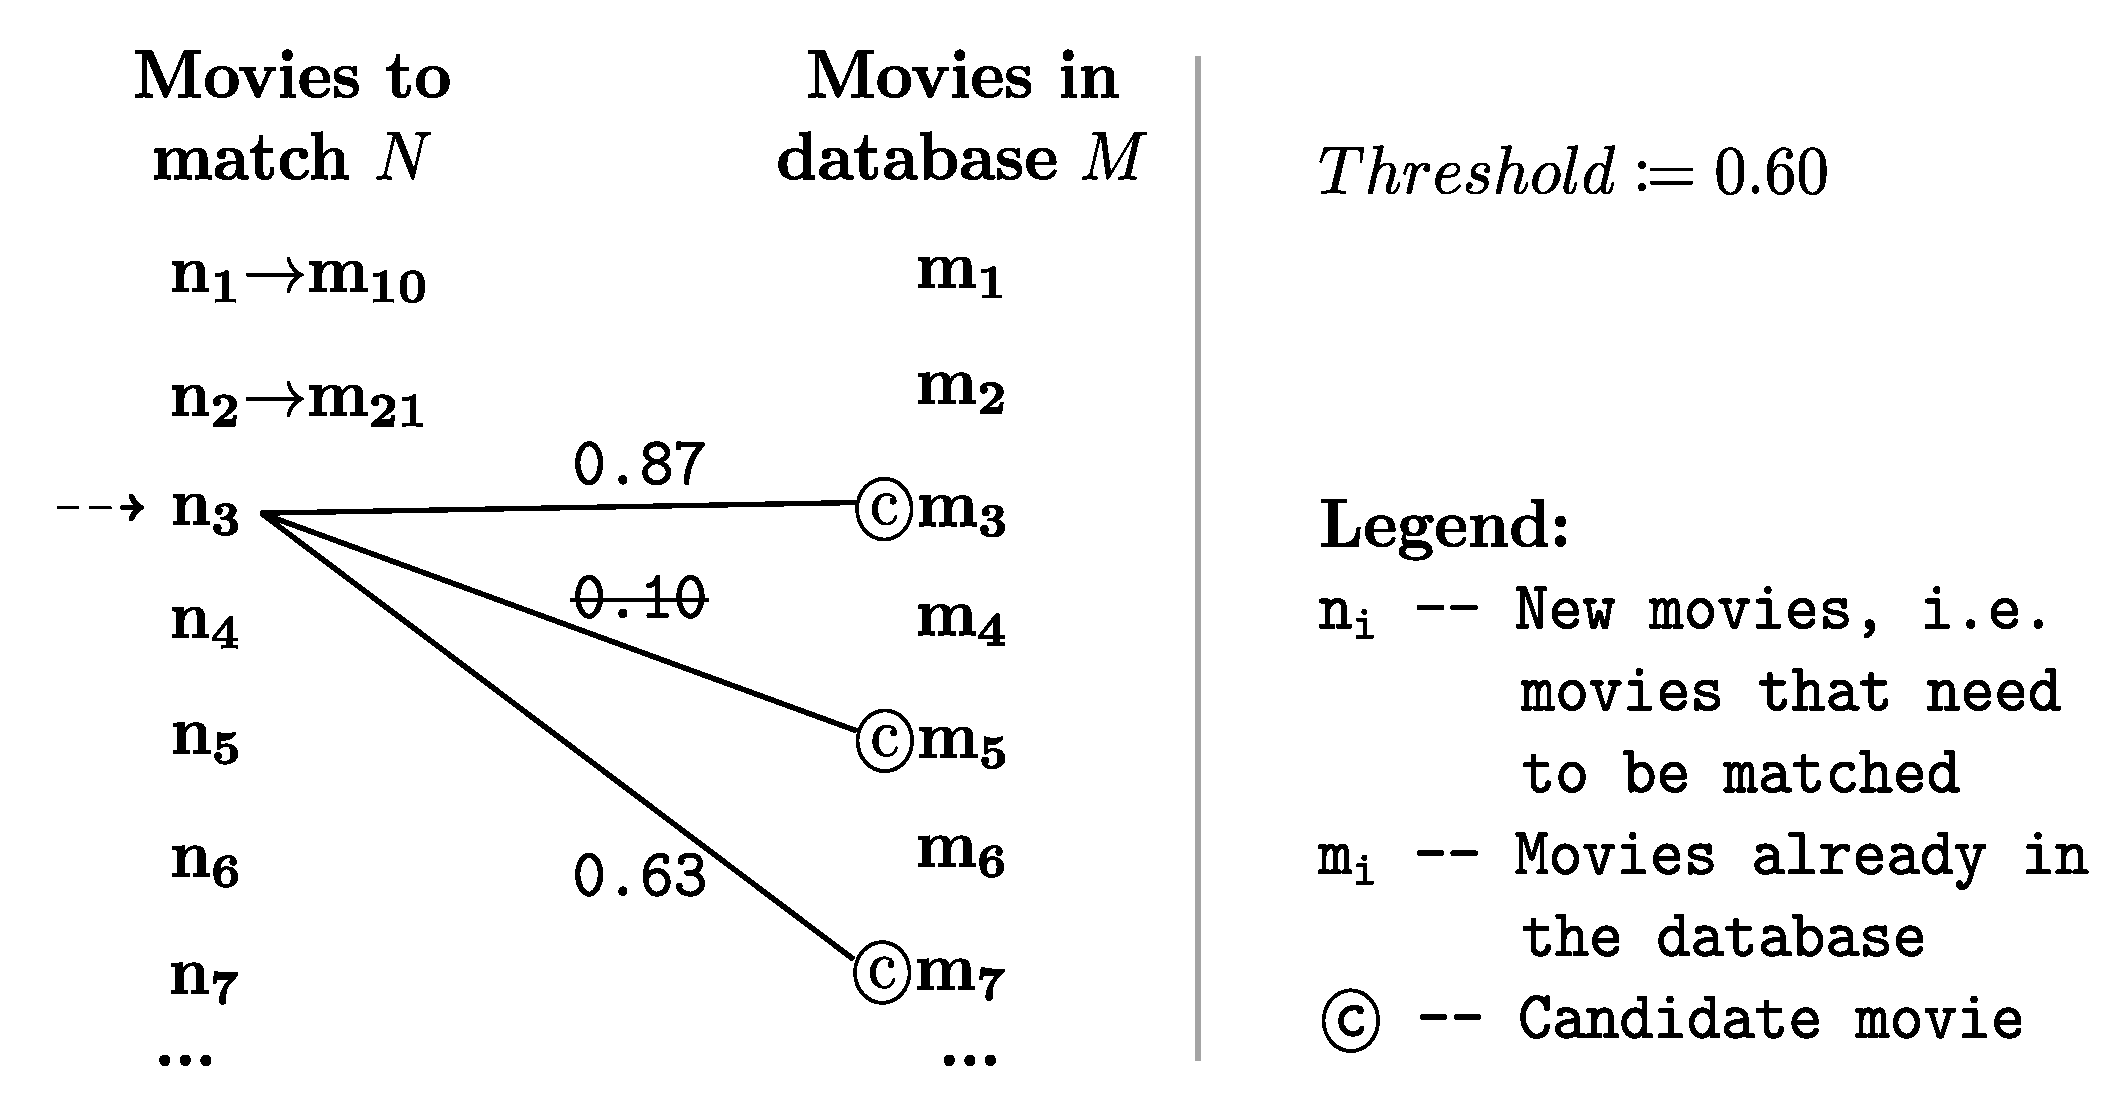
\includegraphics[width=0.8\textwidth]{images/matching_general.pdf}
  \end{center}
  \caption{This shows the general matching procedure. In this case, the algorithm would choose movie $m_3$ as a match for $n_3$, because it has the highest score and is above the threshold.}
  \label{fig_matching_general}
\end{figure}

The next paragraphs describe candidate selection and score calculation in detail.

\paragraph{Candidate selection}

The general goal of candidate selection is to reduce the set of all movies in the database to a smaller set of candidates.
There are two constraints working against each other:
\begin{itemize}
	\item The candidate should be as small as possible. This leads to fewer comparisions and thereby increased performance.
	\item The correct movie, i.e. the movie that needs to be matched to our current movie, must be in the candidate set, if it exists in the database.
\end{itemize}
The former would be optimized by returning nothing, the latter by returning everything, so a viable tradeoff has to be found.

The algorithm presented in this paper uses a candidate selection by calculating a pre-score based on the year and the name of a movie.
This two properties have shown to be available in all datasets for nearly all movies.
The pre-score is calculated based on the Levenshtein distance\footnote{The Levenshtein distance between two strings is defined as the amount of edit operations (insertions, deletions, substitutions), which are needed to transform the first string into the second one.} $n_i$ and each $m_j$ and the distance between the years $year(n_i)$ and $year(m_j)$.
Calculating these numbers for all movies in the database can be done efficient enough to provide a fast candidate selection.
These numbers are combined into a score, where the Levenshtein distance is weighted more.
Finally, the best 100 movies are selected as candidates, according to the score computed in the previous step.

Please note, that candidate selection is not matching over the name, because no decisions need to be made between two similar named movies.
Similar named movies are still good candidates, but the matching itself is using a different approach (see following chapter).

TODO: Reword

\paragraph{Score calculation}
After the candidates have been selected, the next step is to find the best match.
For that, the algorithm uses the actor information, which are available about $n_i$ and each $m_j$ in $C_i$.
Given
\begin{description}
	\item[$n_i$] the movie, which should be matched,
	\item[$C_i$] the set of candidates for the movie,
	\item[$A_{movie}$] a function, which returns the actor names from a movie in one of our datasets,
	\item[$Levenshtein(s_1, s_2)$] a function, which returns the edit distance (insert, remove, replace) between two strings.
\end{description}
the best match $n_i$ is determined as follows:

\begin{align}
	match(n_i) &=
		\begin{cases}
			best\_match(n_i),~if~score > MIN\_SCORE) \\
			\bot
		\end{cases}\label{aoeq:1}\\
	best\_match(n_i) &=
		\argmax_{m_j \in C_i} score(n_i, m_j)\label{aoeq:2}\\
	score(n_i, m_j) &=
		\frac
			{\left\lvert overlap\_set(A_{n_i}, A_{m_j}) \right\rvert}
			{\left\lvert A_{n_i} \right\rvert}\label{aoeq:3}\\
	overlap\_set(A_{n_i}, A_{m_j}) &=
		\Set*{a_n \in A_n}{\exists a_m \in A_m: Levenshtein(a_n, a_m) < ACT\_DIST}.\label{aoeq:4}
\end{align}

The basic idea, which is shown in equation \ref{aoeq:1}, is to only assume a match, if the score of the best matching movie is above a certain threshold $MIN\_SCORE$.
So $MIN\_SCORE$ determines, when a best matching movie is returned as an actual match.
If its score is too low, the assumption is that the movie is not the right one (i.e. the correct one does not exist in the database).
Thus, nothing is returned.

The best matching movie is defined as the movie from the candidate set, which has the highest score (see equation \ref{aoeq:2}).

The algorithm's main idea is illustrated in equation \ref{aoeq:3}: Given the movie to match and a candidate, the score's is determined as the fraction of the movie's actor, which can also be found in the candidate movie's actors.

The check whether one actor from one movie is also in the other movie, there is no use of a strict matching, but rather a fuzzy approach, see \ref{aoeq:4}.
Two actors are considered equal (but only for the sake of matching movies), when their Levenshtein distance is below a certain threshold $ACT\_DIST$.

The main idea of the algorithm is to use the actor overlap between two movies as the main matching criteria.
The Levenshtein distance in \ref{aoeq:4} may not be able to match all actors correctly (i.e. "`Emma Watson"' and "`Emily Watson"' with a distance of three), because similar name problems can occur as with the movie (misspellings, different spelling in different languages, actual similar names for different actors etc.).
However, the idea is that less actors can be matched for different movies and more actors can be matched for the same movie in different data sources.
An evaluation of this approach can be found in section \ref{subsec_evaluation_matching}.

\paragraph{Implementation}
The actual implementation does not only use the actor overlap, but also the overlap for producers, writers and directors.
However, as these sets are usually smaller then the actor set, these overlaps are used with smaller weight than the actor overlap.
Furthermore, the movie name and the year a movie was published is used as the deciding factor between movies, when their actor overlap is equal.

This improvements have shown to produce slightly better results (also see section \ref{subsec_evaluation_matching}).

%!TEX root = ../../lod-group1.tex
\subsection{Updating Movies}
\label{subsec_method_updating}

To ensure that the movies are always up to date, a scheduler is responsible for updating the movies in certain time periods.
The scheduler creates ``CrawlifyMatch'' tasks, which download the movie resource that should be updated, triplifiy it, match it if necessary, and store the updated triples in the triple store.
Thereby, the scheduler distinguishes between existing movies, which were released in the past and upcoming movies, which will be released in the future.

\subsubsection{Adding coming soon Movies}
The steps to add upcoming movies are:
\begin {enumerate}
	\item Get new movie resources.
	\item For each movie, download the new movie resource and triplify it.
	\item Delete all triples of the movie in the triple store in the corresponding graph, if the movie already exists.
	\item Load triples of an IMDb movie into the corresponding graph in the triple store. For the other resources, integrate the triples of the upcoming movie and store them in the corresponding graph.
\end{enumerate}

To get all new movies from IMDb, the scheduler crawls the ``Coming Soon'' page\footnote{\url{http://www.imdb.com/movies-coming-soon/2014-08/}} from the current month until the same month next year.
This page contains all new movies' IDs, which will be released in the crawled time period.
Having the new movie ids, the scheduler can automatically construct the new movie resource\footnote{\url{http://www.imdb.com/[id]}} which can then be crawled.

Freebase has an API, which the scheduler queries for all movies IDs.
Afterwards, the scheduler filters the IDs for unknown IDs.
Thus, the scheduler gets all new movies.

TMDb offers a change set.
The scheduler sends a request to the change API to get all movies which changed recently.
Then, the scheduler can filter for movies which are unknown and thus new.

In OFDb, the movies have increasing IDs.
New movies, added to the database on the current day, can be found on the following page \url{http://www.ofdb.de/view.php?page=neu&Kat=Film&Tage=1}.
So, the scheduler knows the highest and latest movie ID and also the last movie ID of OFDb in the triple store.
All IDs between these two are IDs of new movies.
With the help of these IDs, the scheduler can easily build the URL for the movie resource\footnote{\url{http://www.ofdb.de/film/[id]}} and crawl it.

To figure out how often the scheduler should add upcoming movies, IMDb's upcoming movie list was observed.
The number of upcoming movies added to IMDb each day is shown in Figure \ref{fig_coming_soon_movie}.
On a daily basis, the coming soon page from IMDb was crawled and the changes were recorded.
Almost every day, new movies were added or deleted from the IMDb coming soon list.
It is noticeable, that most movies are published between Thursdays to Sundays on IMDb.

\begin{figure}[h!]
  \begin{center}
  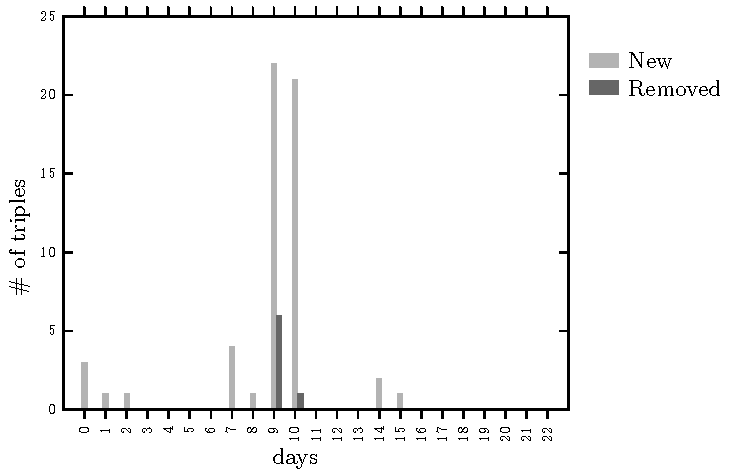
\includegraphics[width=0.8\textwidth]{images/updating_1.pdf}
  \end{center}
  \caption{Number of new upcoming movies, which are published on IMDb per day.}
  \label{fig_coming_soon_movie}
\end{figure}

This observation lead to the decision to update upcoming movies from IMDb on a daily basis.
TMDb and OFDb show similar results, so that upcoming movies from these data sources are updated daily, too.
The sandbox of Freebase, which is requested over the API, updates once a week.
This is why the upcoming movies from Freebase are only updated every week.

\subsubsection{Updating existing Movies}
In Figure \ref{fig_new_movie} the number of changed triples of a newly released movie from IMDb is displayed.
Therefor, a movie was crawled and triplified daily.
Obviously, the movie frequently changes in the first days.
Also, the number of changing triples decreases with time.
Triples changing often are mostly cast triples, links to images and videos, IMDb rating, character triples or taglines.

\begin{figure}[h!]
  \begin{center}
  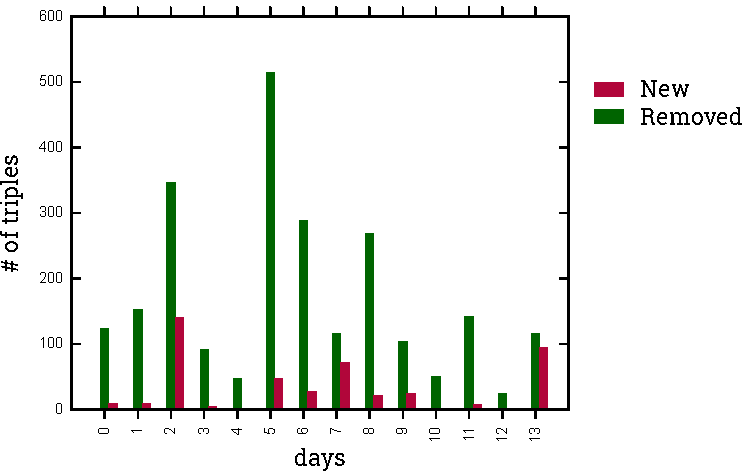
\includegraphics[width=0.8\textwidth]{images/updating_2.pdf}
  \end{center}
  \caption{Number of triples, which change in the first days of a newly released movie from IMDb.}
  \label{fig_new_movie}
\end{figure}

Because a movie changes less the older it is, existing movies are divided into different categories.
Each category is updated at different frequencies (Table \ref{tab_updating_existing}).
\begin{table}[ht]
	\begin{center}
	\begin{tabular}{rl}
		\textbf{Category of movie} & \textbf{Frequency} \\ \hline
		one year old & weekly \\
		5 year old & monthly \\
		5 - 25 years old & yearly \\
		older than 25 years & never \\
	\end{tabular}
	\end{center}
	\caption{Frequency of updating existing movies}
	\label{tab_updating_existing}
\end{table}
If a category should be updated, the scheduler does the following steps:
\begin{enumerate}
	\item Find all movies which should be updated regardless their original data source.
	\item For each of these movies, get the updated movie resource and triplify it.
	\item Delete all triples of the movie in the triple store in the corresponding graph.
	\item Load the new triples into the corresponding graph in the triple store.
\end{enumerate}
Because the movies are stored in different graphs depending on their original data source, the scheduler knows where to find the movie resource in the web.
The original resource of a movie is stored in a \emph{sameAs} triple.
Deleting the existing triples and storing the newly downloaded triples ensures that no conflicting information of a resource is stored.
\newpage
\section{Evaluation}
\label{sec_evaluation}

The following sections explain the evaluation process of matching and updating

%!TEX root = ../../lod-group1.tex
%\subsection{Matching}
\label{subsec_evaluation_matching}

\subsection{Introduction}
The matching algorithm, explained in Section \ref{subsec_method_matching}, depends on multiple parameters.
The following paragraphs explain the process of tuning these parameters and evaluating the quality of the matching algorithm.

Evaluation is done on two sets of 4000 randomly selected movies.
The selection is done by listing all movies sorted by name and then using $Random.shuffle$ to shuffle the list and take the first 4000 movies.
The first list is used for the parameter optimization, while the second is used for the final evaluation.
To get a gold standard, only those movies with an annotated IMDb-ID are taken into consideration.
However, the ID is not used to match the movies, it is only used as the gold standard.
These movies can be split into two parts: the movies that could potentially be matched and the movies that cannot be matched, i.e. movies that do not exist in the database.
The result is two lists of around 3000 movies which are then used to test the algorithm.
Around 2000 of these movies could possibly be matched.

Evaluation itself is done by means of precision, recall and F0.5-measure.
As explained in Section \ref{subsec_method_matching}, Precision is more important and therefore the F0.5-measure is additionally observed in the evaluation process.
The following paragraphs show the definitions of the relevant sets for the purpose of calculating these evaluation metrics.

Given the set of new movies $N$ and the set of existing movies $M$ the following function returns the correct matching movie $m_{j} \in M$ of a new movie $n_{i} \in N$:

\begin{align}
	gold: ~&N \rightarrow M \cup \{\bot\} \\
	gold(n) &=
		\begin{cases}
		m \in M ~\text{if matching movie m exists in database}  \\
		\bot
		\end{cases}
\end{align}

The function $gold$ is defined by looking at the IMDb-IDs as described above.
Using this function and the algorithm $match_{n_{i}}$ explained in \ref{subsec_method_matching} the following sets are defined:

\begin{description}
\item[True Positives (TP)] is the set of correct matches between a new movie and an existing one in the database,
\begin{align}
TP &\coloneqq \Set*{(n_i, match(n_i))}{match(n_i) = gold(n_i) \land match(n_i) \neq \bot}
\end{align}
\item[False Positives (FP)] is the set of incorrect matches, either meaning another movie is the correct match or no correct match exists in the database
\begin{align}
FP &\coloneqq \Set*{(n_i, match(n_i))}{match(n_i) \neq gold(n_i) \land match(n_i) \neq \bot}
\end{align}
\item[True Negatives (TN)] is the set of tuples that are no matches and that cannot be matched because they are not in the database,
\begin{align}
FP &\coloneqq \Set*{(n_i, m_j)}{m_j \in M \land (m_j \neq match(n_i) \land m_j \neq gold(n_i) \lor m_j = \bot)}
\end{align}
\item[False Negatives (FN)] is the set of correct matches between movies that have not been found.
\begin{align}
FP &\coloneqq \Set*{(n_i, m_j)}{m_j \in M \land m_j \neq match(n_i) \land m_j = gold(n_i) \land m_j \neq \bot}
\end{align}
\end{description}

Based on these sets, standard definitions of the evaluation metrics, precision, recall, and F0.5-measure are used.

To generate consistent results, the whole evaluation is done without the distributed environment, as explained in Section \ref{subsec_method_architecture}, but on a single machine with the following system specifications:
\begin{itemize}
	\item CPU: Pentium(R) Dual-Core  CPU E5300  @ 2.60GHz
	\item RAM: 16GB, Java is run with 4GB of RAM
	\item OS: Debian 3.2.57
\end{itemize}

The evaluation process is structured into two parts: parameter optimization and final evaluation.
In the first part, several experiments were conducted regarding the optimal parameters.
Concretely, the goal was to find good values for $ACT\_DIST$, $MIN\_SCORE$ and $CANDIDATE\_SET\_SIZE$.
In the second part, the algorithm will be evaluated on the second dataset against the baseline approach of matching by name.
Furthermore, to evaluate the bias of using the annotation of IMDb-IDs as gold standard, the algorithm was run on a set of 100 movies that do not have an IMDb-ID annotated and the results are compared to a handcrafted gold standard.

TODO: List of annotated properties

TODO: Important, how are the other parameters set?

\subsection{$CANDIDATE\_SET\_SIZE$ parameter}
The first test looks at the impact on the quality of the results when the number of considered candidates is increased (see Figure \ref{fig_candidate_set_size}).
For each test step, the candidate set size was doubled (starting at 2), hence a logarithmic scale is used.
In general, the candidate set size should be as small as possible, because the greater this number, the longer the runtime of the matching process.
For example, when trying to match 4000 movies, it takes 145 minutes with a $CANDIDATE\_SET\_SIZE$ of 1024, but 276 minutes with a $CANDIDATE\_SET\_SIZE$ of 2048.

\begin{figure}[h!]
  \begin{center}
  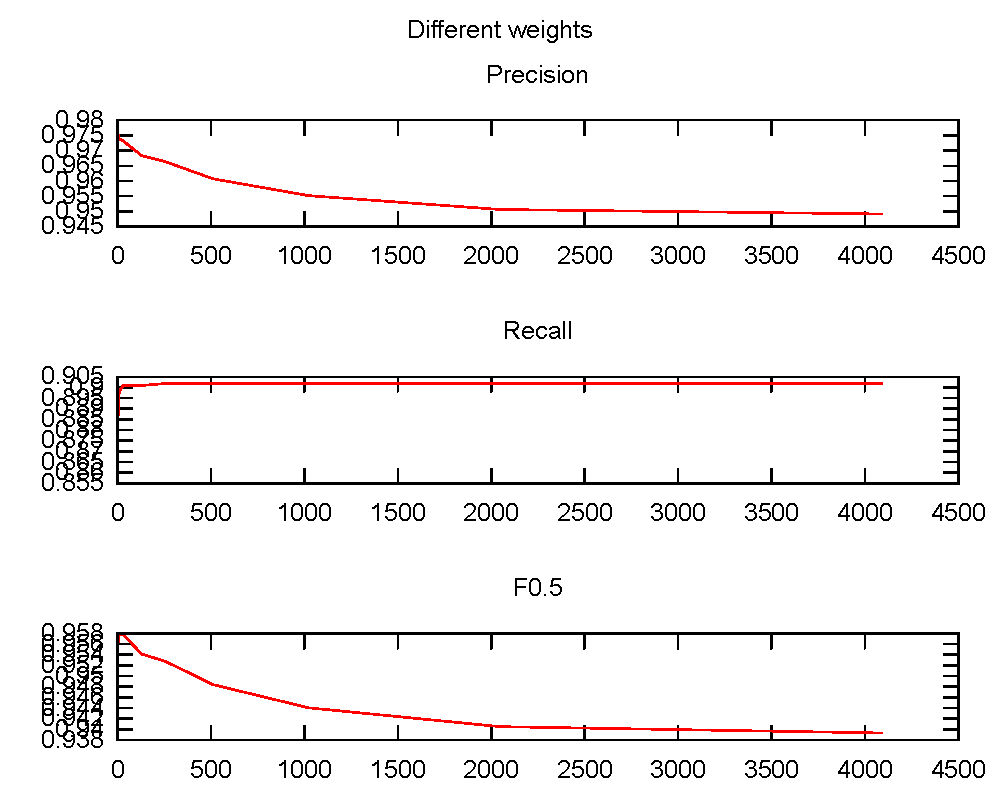
\includegraphics[width=0.8\textwidth]{images/candidateSetSize.pdf}
  \end{center}
  \caption{$CANDIDATE\_SET\_SIZE$ evaluation: The best F0.5 performance is reached at a candidate set size of 32.}
  \label{fig_candidate_set_size}
\end{figure}

\subsection{$ACT\_DIST$ and $MIN\_SCORE$ parameter}
A second test observes the maximum Levenshtein distance between two actors and the threshold that needs to be reached for the actor overlap.
The assumption is, that these parameters are not independent of each other, as both directly affect the scoring procedure.
Increasing $ACT\_DIST$ immediately leads to a higher score, because more actors are considered the same.

For the optimization, $ACT\_DIST$ was tested for values from 1 to 4 and $MIN\_SCORE$ was tested for every value from 0 to 1 in 0.1 steps.

The results can be seen in Figure \ref{fig_3d}.
The results for $MIN\_SCORE > 0.7$ and $MIN\_SCORE < 0.1$ are far worse than the other results, which is why they have been excluded from the figure.
The optimal value is at $MIN\_SCORE = 0.2$ and $ACT\_DIST = 2$.

\begin{figure}[h!]
  \begin{center}
  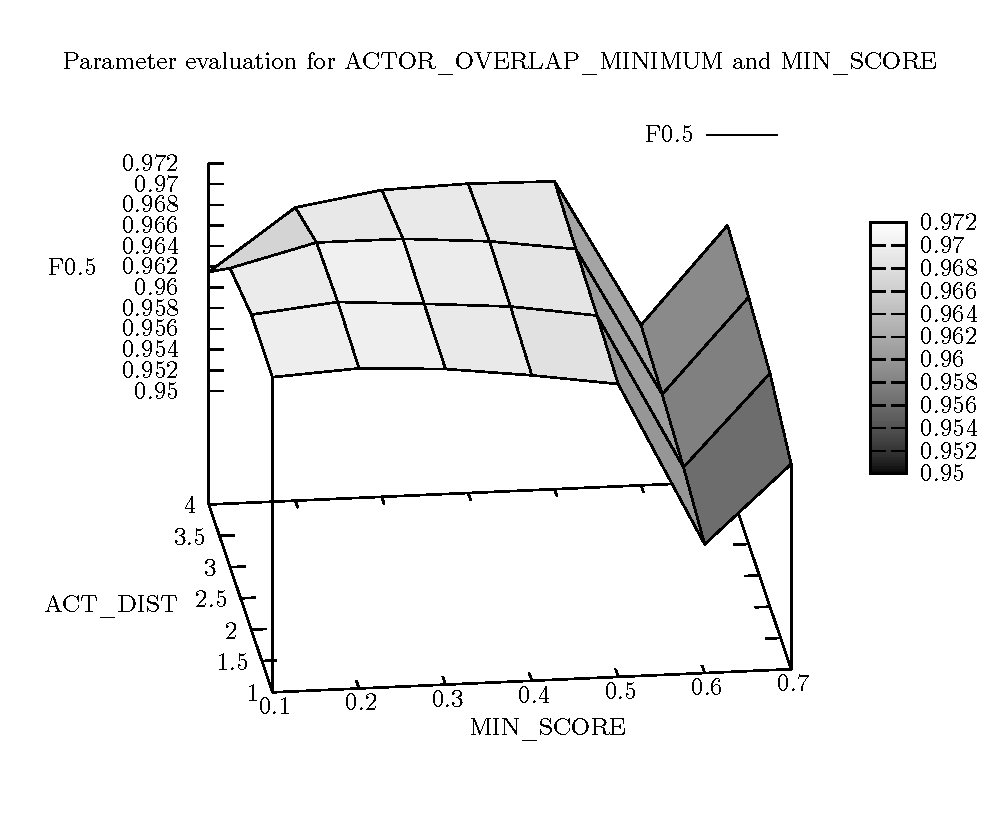
\includegraphics[width=0.8\textwidth]{images/3d.pdf}
  \end{center}
  \caption{$ACT\_DIST$  and $MIN\_SCORE$ evaluation. There are a lot of false positives between a threshold of 0.6 and 0.7, which explains the knee.}
  \label{fig_3d}
\end{figure}


% \subsection{Refinement Weight}

% \begin{figure}[h!]
%   \begin{center}
%   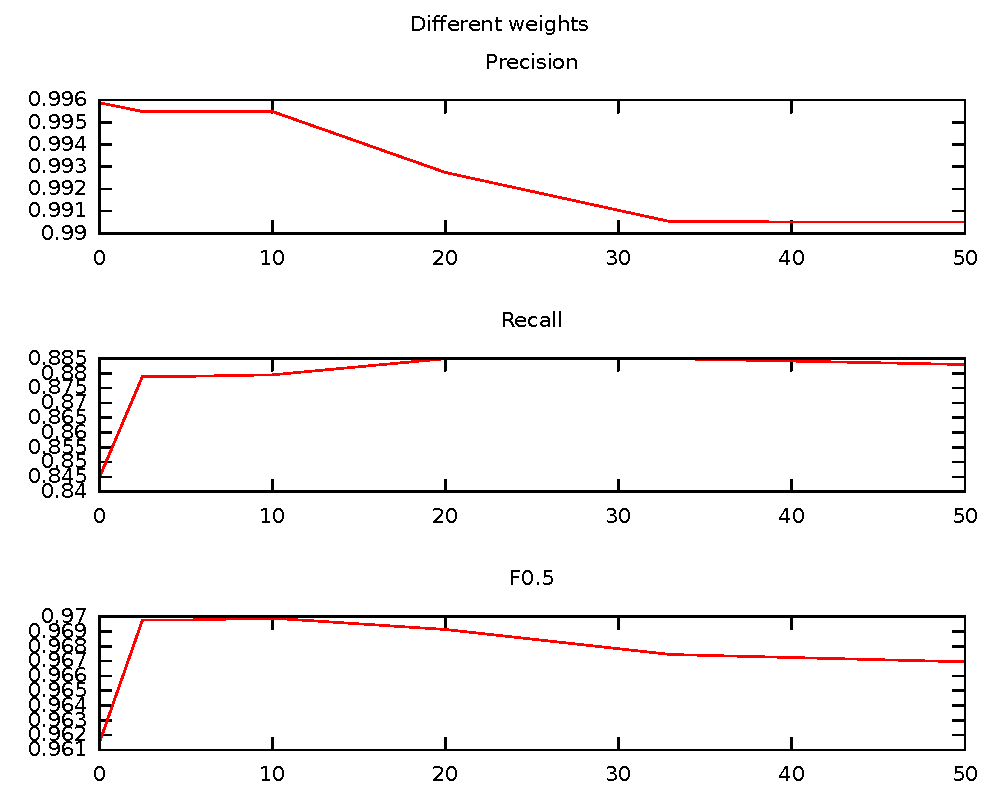
\includegraphics[width=0.8\textwidth]{images/graph_weight.pdf}
%   \end{center}
%   \caption{Refinement weight}
%   \label{fig_weight}
% \end{figure}
\subsection{Final Evaluation}
With the determined parameters $MIN\_SCORE = 0.2$, $ACT\_DIST = 2$ and $CANDIDATE\_SET = 32$ the evaluation ran on the two other test sets as described above.
The final results are shown in Figure \ref{fig_baseline}.
For comparison, the results of the baseline approach are shown as well.
The baseline approach matches if there is an exact match between any of the annotated names of the new movie and the annotated names of a movie in the database.

\begin{figure}[h!]
  \begin{center}
  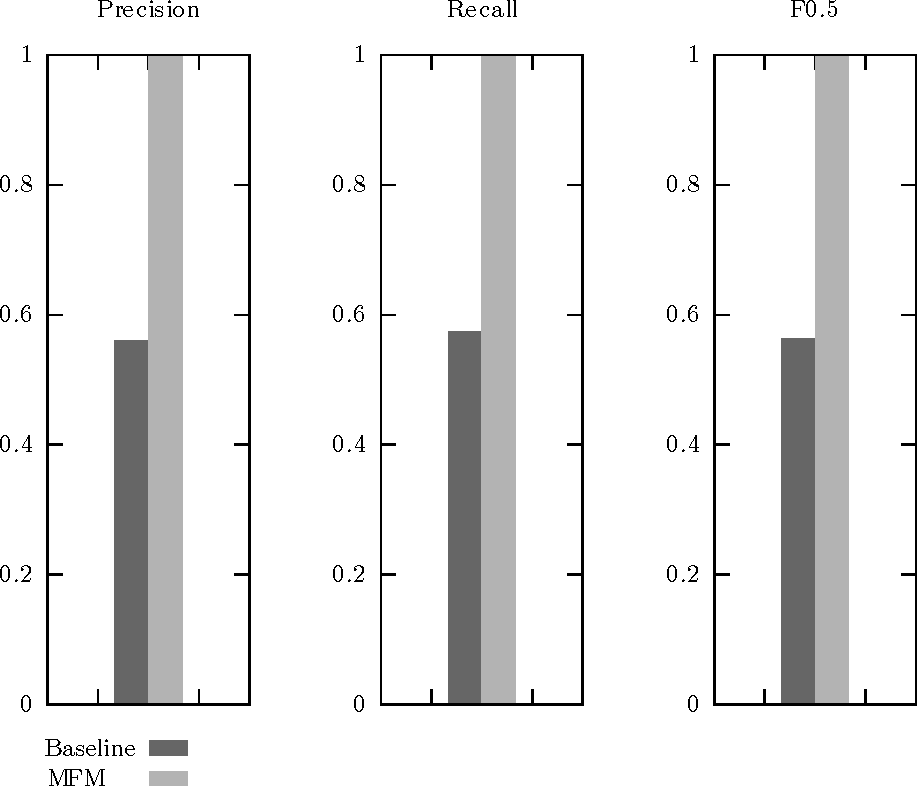
\includegraphics[width=0.8\textwidth]{images/baseline.pdf}
  \end{center}
  \caption{TODO}
  \label{fig_baseline}
\end{figure}

\subsection{Error Sources}
An error analysis was conducted and the results are listed in the following paragraph.

In general, if the systems returns a match, this is very likely to be correct, as indicated by the high precision.
In the cases, where an incorrect match was returned, this was most likely a match for a movie, which was not in the database, i.e. the system found a match from the database, but actually, there was no correct match.
This was the case in 85\% of the returned incorrect matches.
The remaining 15\% were actual wrong matches, i.e. the correct movie could have been found, but wasn't.

The bigger problem was not finding a possible match.
For this, the following error sources have been identified:

\begin{itemize}
	\item
    In around 70\% of the cases, a match was not found because the correct match was not in the candidate set
	\item
    In around 20\% of the cases, the information used for matching was not available.
    In general, lots of movies without an IMDb-ID only have a name and an overview (free text).
	\item
    In the remaining cases, the correct movie would have been matched but the calculated score was lower then the threshold.
\end{itemize}

%!TEX root = ../../lod-group1.tex
\subsection{Updating}
\label{subsec_evaluation_updating}

The scheduler, described in Chapter \ref{subsec_method_updating}, updates movies at certain times.
Thereby, the scheduler distinguish between existing and coming soon movies.

How many coming soon movies are daily added to IMDb is shown in Figure \ref{fig_coming_soon_movie}.
On a daily basis, the coming soon page from IMDb was crawled and the changes were recorded.
Almost every day, new movies are added or deleted from the IMDb coming soon list.
It is noticeable, that the most movies are published between Thursdays to Sundays on IMDb.

\begin{figure}[h!]
  \begin{center}
  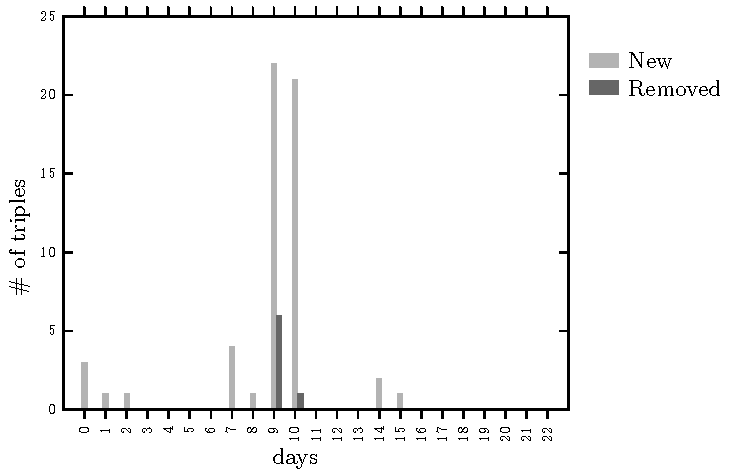
\includegraphics[width=0.8\textwidth]{images/updating_1.pdf}
  \end{center}
  \caption{Number of new coming soon movies, which are published on IMDb per day.}
  \label{fig_coming_soon_movie}
\end{figure}

In Figure \ref{fig_new_movie} the number of changed triples of a new released movie from IMDb is displayed.
Therefor, the movie was crawled and triplified daily.
As you can seen, the movie frequently changes in the first days.
Often changing triples are for example cast triple, links to images and videos, IMDb rating, charachter triples or taglines.

\begin{figure}[h!]
  \begin{center}
  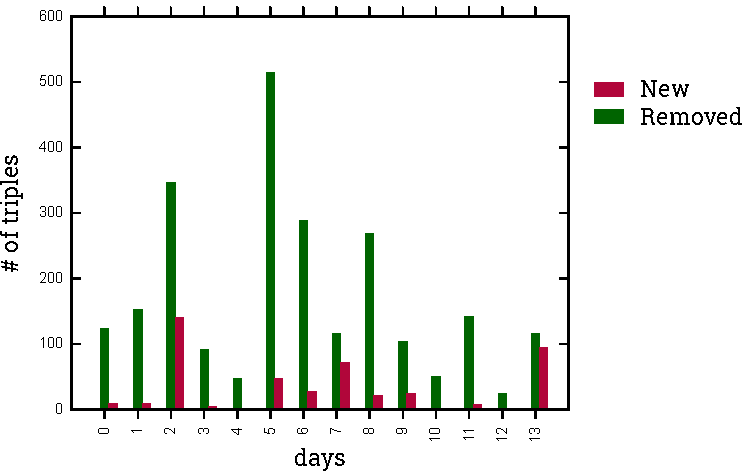
\includegraphics[width=0.8\textwidth]{images/updating_2.pdf}
  \end{center}
  \caption{Number of triples, which change in the first days of a new released movie from IMDb.}
  \label{fig_new_movie}
\end{figure}
\newpage
%!TEX root = ../lod-group1.tex
\section{Discussion of Evaluation Results}
\label{sec_discussion}

The results shown in Section \ref{sec_evaluation} give a lot of insight on the used approach.
The following section will discuss these findings and give insight on conclusions and possible improvements.

Figure \ref{fig_baseline} shows the huge improvement of the discussed algorithm to the baseline approach.
This improvement can be explained by the limiting factors of the baseline approach, which have already been explained in Section \ref{subsec_method_matching}.

On the other hand, Figure \ref{fig_baseline} also shows results for matching movies with no IMDb-ID annotated.
When comparing this with the results from movies, which have an IMDb-ID annotated, a bias is clearly visible.
Both precision and recall are significantly lower.
This can be explained by the general lower annotation quality of those movies.
Some movies even only have a name, with no further data annotated.
However, compared to the baseline approach it is still a good improvement.

Even though the results are already good there is still room for better results.
The analysis of the wrongly matched movies and the not found matches, as listed in Section \ref{subsec_evaluation_matching} has shown that the biggest possible gain is in improving the way the candidates are selected.
Since candidate selection is based only on the name and the year at the moment, movies with names that are not annotated so far are most likely not found.
Thus, further criterias should be considered when calculating the pre-score for selecting candidates.
Especially a set of movies that is choosen without an influence of there name could help.
However, the movies that need to be matched, i.e. the one that do not have an annotated IMDb-ID, usually have many other properties not annotated.
Possible further attributes to consider are overview, runtime and genre.
Nonetheless, non of them are trivial to integrate.

surprisingly, wird nicht besser wenn candidate set size groesser -> erklaeren

discuss: cartoons, evaluation


\newpage
%!TEX root = ../lod-group1.tex
\section{Conclusion and Outlook}
\label{sec_conclusion}

\emph{Match Forrest, Match!} is a system which combines various information from different data sources to a unified, linked open data set of movies.
The system is based on the main data source \textit{IMDb}, which has extensive information of movies.
The information from this data source were enriched which data from other data sources.
By it, highly attention was payed to the consistency and correctness of the matched data.

In the future the system could include more data sources.
For example a data source, which contains Indian movies, would be useful to expand the number and range of movies.
Also, the system should be connected to \textit{DBpedia} in the future, because \textit{DBpedia} is the core of the semantic web.

Besides, the system could also include other resources as movies, such as TV films or TV series.

Further more, it would be helpful for users, which want to search for movies only knowing some plot points, to build a website which allows easy searching.

To ensure that movies from different data sources are matched correctly, the matching algorithm could be improved further.
Also, the merging of movies could be enhanced.


%% Anhänge
\newpage
\begin{appendix}


%!TEX root = ../lod-group1.tex
\section{Glossary} %Appendix (Glossar)


\begin{description}
\item[Browser:]\index{Browser} blabla
\end{description}


\newpage

% Appendix (Akronyme)
\section{Abbreviations and Acronyms}\index{Acronyms}

\begin{tabbing}
\hspace*{3cm}\=  \\ \kill
WWW \> World Wide Web\\
\end{tabbing}


\end{appendix}


%Hier kommt das Literaturverzeichnis
\newpage

\addcontentsline{toc}{section}{References} % Zeile für das Inhaltsverzeichnis

\bibliography{bibfile}
\bibliographystyle{alphadin}

\newpage

%Hierhin kommt der Index (Sachverzeichnis)
%\addcontentsline{toc}{section}{Index} % Dies ist die Zeile für das Inhaltsverzeichnis
%\flushbottom
%\printindex

\end{document}
